\documentclass[11pt,tightenlines,nofootinbib,superscriptaddress,notitlepage, APS, pra]{beamer}

%\usepackage[auth-sc]{authblk}
%\usepackage{fullpage}
\usepackage{appendix}
\usepackage[inkscape={/Applications/Inkscape.app/Contents/Resources/bin/inkscap‌​e -z -C}]{svg}
%\usepackage{geometry}
%\renewcommand{\abstractname}{}}
\def \ooo{\o}
%%%%%%%%% PACKAGES %%%%%%%%%
%\bibliographystyle{apsrev4-1.bst}
\usepackage{amsfonts,amssymb,amstext,amsmath,amsthm}
%\usepackage{MnSymbol}
\usepackage{graphicx}
%\usepackage{subcaption}
\usepackage{mathtools}
%\usepackage{epstopdf}
%\usepackage{epsfig}
%\usepackage{pstool}
%\usepackage{latexsym}
%\usepackage{psfrag}
%\usepackage{amsfonts}
%\usepackage{bm} % bold math
%\usepackage{txfonts, pxfonts}
%\usepackage{bbm}
\usepackage{showlabels}
%\usepackage{fancyhdr}
%\usepackage{axodraw}
\usepackage{color}
\usepackage{hyperref}
%%% MINE %%%
\usepackage{float}
\usepackage{placeins}
\usepackage{bbold}
\usepackage{indentfirst}
\usepackage{tabu}
\usepackage{verbatim}
\usepackage{comment}
\usepackage{enumerate}

\theoremstyle{definition}
\newtheorem{mydef}{Definition}
\theoremstyle{plain}
\newtheorem{lem}{Lemma}
\newtheorem{thm}{Theorem}
\newtheorem{cor}{Corollary}
\newtheorem{prop}{Proposition}

\usepackage{relsize}

%%%%%%%%% MARGINS %%%%%%%%%%

%\setlength{\topmargin}{0.5cm}
%\setlength{\textheight}{22cm}
%\setlength{\textwidth}{16cm}
%\setlength{\evensidemargin}{-0.5cm}
%\setlength{\oddsidemargin}{-0.5cm}


%%%%%%%%% ENVIRONMENTS %%%%%%%%%%

\newcommand{\be}{\begin{equation}}
\newcommand{\ee}{\end{equation}}
\newcommand{\barray}{\begin{array}}
\newcommand{\earray}{\end{array}}
\newcommand{\bea}{\begin{eqnarray}}
\newcommand{\eea}{\end{eqnarray}}
\newcommand{\bs}{\begin{subequations}}
\newcommand{\es}{\end{subequations}}
\newcommand{\balign}{\begin{align}}
\newcommand{\ealign}{\end{align}}
\newcommand{\equ}{\begin{equation}}
\newcommand{\nequ}{\end{equation}}
\newcommand{\eqa}{\begin{eqnarray}}
\newcommand{\neqa}{\end{eqnarray}}

 
 
 %%%%%% COMMANDS %%%%%%
 
\def\nn{\nonumber}
\newcommand{\Ref}[1]{(\ref{#1})}

\newcommand{\re}{\mathrm{Re}}
\newcommand{\im}{\mathrm{Im}}

\newcommand{\bra}[1]{\la {#1}|}
\newcommand{\ket}[1]{|{#1}\ra}
\newcommand{\mean}[1]{\la{#1}\ra}
\newcommand{\id}{\mathbbm{1}}

\newcommand{\mrm}[1]{\quad \mathrm{#1}\quad}
\def \interior {\mathlarger{\mathlarger{\lrcorner}}\,}

%%%%%%%%% Greek-SYMBOLS %%%%%%%%%%
\def\ka{\kappa}
%\def\om{\omega}
\def\Ga{\Gamma}
\def\ga{\gamma}
\def\sig{\sigma}
\def\ph{\varphi}
\def\eps{\epsilon}
\def\th{\theta}
\def\Th{\Theta}
\def\al{\alpha}
\def\d{\delta}
\def\lam{\lambda}
\def\o{\omega}
\def\vareps{\varepsilon}
\def\a{\alpha}
\def\b{\beta}
\def\g{\gamma}
\def\eps{\epsilon}
\def\bphi{\bm\varphi}
\def\brd{\bm\rd}
\def\bj{\bm j}
\def\bpi{\bar{\pi}}
\def \rb {\right)}
\def \lb {\left(}
\def\da{{\dot{\alpha}}}
\def\db{{\dot{\beta}}}
\def\dg{{\dot{\gamma}}}
\def\dm{{\dot{\mu}}}
\def\dn{{\dot{\nu}}}
\def\pa{\phantom{\alpha}}
\def\bs{\bar{\sigma}}
\def\bl{\bar{\lambda}}
\def\bp{\bar{\pi}}
\def \v {{v}}
\def \vpos {{\hat{v}}}
\def \pap {\phantom{\alpha'}}
\def \xh {{\hat{x}}}
\def \bri {{(i)}}
\def \brj {{(j)}}
\def \bone{{(1)}}
\def \btwo {{(2)}}
\def \bthr {{(3)}}
%\def \mp {{\mu'}}



\newcommand{\om}{\ominus}
\newcommand{\op}{\oplus}


%%%%%%% Derivatives %%%%%%%%%

\newcommand{\rd}{\mathrm{d}}
\newcommand{\p}{\partial}
\newcommand{\N}{\nabla}
\def\cL{ {\cal L}}
\def\i{\imath}

%%%%%%% MATH-SYMBOLS%%%%%%


\def\bra{\langle}
\def\ket{\rangle}
\def\lb{\left\lbrace}
\def \rb{\right\rbrace}
\def\w{\wedge}
\def\f{\frac}
\def\i{\imath}
%\def\ot{\check{t}}
\def\ot{{t^{\perp}}}
\def\htt{\hat{t}}
\def\bS{\bar{\Sigma}}
\def\sl2c{SL(2,\mathbb{C})}
\newcommand{\vect}[1]{\left\vert #1 \right\rangle}
\newcommand{\covec}[1]{\left\langle #1 \right\vert}
\newcommand{\inner}[1]{\langle #1 \rangle}
\newcommand{\mc}[1]{\mathcal{#1}}
\newcommand{\mf}[1]{\mathfrak{#1}}
\newcommand{\oprod}[2]{\left\vert #1\right\rangle\left\langle #2\right\vert}
\newcommand{\pair}[1]{\left\langle #1\right\rangle}
\newcommand{\abs}[1]{\vert #1 \vert}
\newcommand{\com}[1]{\left[#1\right]}
\newcommand{\pb}[1]{\left\lbrace #1 \right\rbrace}
\newcommand{\overbar}[1]{\mkern 1.5mu\overline{\mkern-1.5mu#1\mkern-1.5mu}\mkern 1.5mu}
\newcommand{\TT}[2]{T_{#1}#2}
\newcommand{\Ad}[1] {\mathrm{Ad}_{#1}}
\newcommand{\clam}[1]{\bar{\lambda}^{\dot{#1}}}
\newcommand{\clamd}[1]{\bar{\lambda}_{\dot{#1}}}
\newcommand{\cpi}[1]{\bar{\pi}_{\dot{#1}}}
\newcommand{\cpiu}[1]{\bar{\pi}^{\dot{#1}}}
\def \Tr {\mathrm{Tr}}
\def \tr{\mathrm{tr}}
\def \Ad{\mathrm{Ad}}
\def \ad{\mathrm{ad}}
\def \hp{\hat{P}}
\def \hj{\hat{J}}
\def \hx{\hat{X}}
\def \hc{\hat{C}}


%%%%TILDE-BAR-underline%%%%
\def\bs{\bar{s}}
\def\bn{\bar{n}}
\def\bbn{\bm{\bar{n}}}
\def\bbs{\bm{\bar{s}}}
\def\bhr{\bm{\hat{r}}}
\def\aa{\bm{a}}
\def\bb{\bm{b}}
\def\bbb{\bm{\bar{b}}}
\def\aaa{\bm{\bar{a}}}
\def\bom{\bar{\omega}}


\def\tl{\tilde}
\def\tn{\tilde{n}}
\def\tz{\tilde{z}}
\def\wtl{\widetilde}
\newcommand{\vj}{\vec{\jmath} }
\newcommand{\tP}{\tilde{P} }
\def\tg{\tl{g}}
\def\tM{\tl{M}}
\def\tz{\tilde{z}}
\def\tX{\tilde{X}}
\def\bz{\bar{z}}

\newcommand{\un}[1]{\underline{\bm{#1}}}
\newcommand{\ov}[1]{\overline{#1}}

%%%%%%%%BOld%%%%%%%%
\def\n{\bm{n}}
\def\t{\bm{t}}
\def\K{\bm{K}}
\def\s{\bm{s}}
\def\r{\bm{r}}
\def\u{\bm{u}}
\def\bht{\bm{\hat{t}}}
%\def\bot{{\bm{\check{t}}}}
\def\bot{\bm{t^{\perp}}}
\def\bxi{\bm{\xi}}
\def\dd{\!\cdot \!}
\def\bmo{\bm{\omega}}
\newcommand{\mbf}[1]{\mathbf{#1}}
\newcommand{\mbg}[1]{\boldsymbol{#1}}


%%%%%%%%% MATHBB_CAL %%%%%%%%%%

\newcommand{\NN}{\mathbb{N}}
\newcommand{\Z}{\mathbb{Z}}
\newcommand{\Q}{\mathbb{Q}}
\newcommand{\R}{\mathbb{R}}
%\DeclareMathOperator{\tr}{Tr}
\newcommand{\hh}{{\cal H}}
\newcommand{\oo}{{\cal O}}
\newcommand{\cs}{{ S}}
\usepackage{bbm}
\def\Id{{\mathbbm 1}}
\def\C{{\mathbbm C}}
\def\R{{\mathbbm R}}
\def\Z{{\mathbbm Z}}
\newcommand{\SU}{\mathrm{SU}}
\newcommand{\SO}{\mathrm{SO}}
\newcommand{\SL}{\mathrm{SL}(2,\mathbb{C})}
\newcommand{\su}{\mathfrak{su}}
\newcommand{\so}{\mathit{so}}
\newcommand{\bg}{{\mathbf g}}
\newcommand{\LX}{{\cal L}_{\hat X}}
\def\Ee{{\cal E}}
\def\kk{{\cal K}}
\def\cS{{\cal S}} 
\def\g{\mathfrak{g}}
\def\gg{\mathfrak{g}^*}
\def\p{\mathfrak{p}}
\def\pp{\mathfrak{p}^*}
\def\pw{\mathfrak{pw}}
\def\pwd{\mathfrak{pw}^*}
\newcommand{\mr}[1]{\mathrm{#1}}

%%%% SIZE %%%%

\newcommand{\scr}{\rm\scriptscriptstyle}
\newcommand{\fsize}{\footnotesize}


%%%% TIKZ %%%%
\usepackage{tikz}
\usetikzlibrary{backgrounds}
\usetikzlibrary{decorations.pathmorphing}
\usetikzlibrary{decorations.pathreplacing}
\usepackage{tkz-euclide}
\usetikzlibrary{decorations.markings}
\tikzset{->-/.style={decoration={
  markings,
  mark=at position .5 with {\arrow{>}}},postaction={decorate}}}

\usetikzlibrary{decorations.markings, shapes.geometric}
\tikzstyle{Box1} = [rectangle, rounded corners, minimum width=3cm, minimum height=1cm,text centered, draw=none, fill=red!60!black]
\tikzstyle{Box2} = [diamond, rounded corners, minimum width=3cm, minimum height=1cm,text centered, draw=none, fill=green!60!blue]
\tikzstyle{Box3} = [rectangle, rounded corners, minimum width=3cm, minimum height=1cm,text centered, draw=none, fill=blue!60!green]
\tikzstyle{every picture}+=[remember picture]
\usetikzlibrary{shapes.multipart}
\usetikzlibrary{positioning}
\usetikzlibrary{calc, 3d, decorations}
%\everymath{\displaystyle}
\tikzstyle{na} = [baseline=-.5ex]
\setbeamerfont{footnote}{size=\scriptsize}

%\newcommand{\tr}{{\mathrm{Tr}}}
\usetheme{Madrid}
\usecolortheme{whale}
\usefonttheme{serif}
\beamertemplatenavigationsymbolsempty
\title[Taxi Data]{Life in New York City as Told by Taxis}
\author[T.Rempel]{Trevor~Rempel}
\institute[PI]{Perimeter Institute and University of Waterloo}
\date[Data Incubator]{\today}
\hypersetup{
    colorlinks=true,
    linkcolor=blue,
    filecolor=magenta,      
    urlcolor=cyan,
}
\usepackage[font={small}]{caption}
\setbeamertemplate{caption}[numbered]

%gets rid of bottom navigation bars
\setbeamertemplate{footline}[frame number]{}

%gets rid of bottom navigation symbols
\setbeamertemplate{navigation symbols}{}

%gets rid of footer
%will override 'frame number' instruction above
%comment out to revert to previous/default definitions
%\setbeamertemplate{footline}{}


%%%%%%%%%%%%%%%%%%%%%%%%%%%%%%%%%%%%%%%%%%%%%%%%%%%%%%%%%%%%%%%%%%%%%%%%%

\begin{document}

\setbeamertemplate{enumerate items}[default]

\frame{\titlepage}
\setbeamertemplate{section in toc}[circle]
\begin{frame}
\frametitle{Table of Contents}
\tableofcontents
\end{frame}
\AtBeginSection[]{
  \begin{frame}
  \vfill
  \centering
  \begin{beamercolorbox}[sep=8pt,center,shadow=true,rounded=true]{title}
    \usebeamerfont{title}\secname\par
  \end{beamercolorbox}
  \vfill
  \end{frame}
}


\section{Introduction}
\graphicspath{{/Users/tjrempel/dataIncubator/Analysis/}}
\begin{frame}{Introduction}
What is it like to live in New York City? Often one turns to social media data:
\begin{itemize}
\item Blog Posts
\item Facebook
\item Twitter
\item Yelp
\end{itemize}
Obtain an alternative perspective by considering \href{http://www.nyc.gov/html/tlc/html/about/trip_record_data.shtml}{data} on taxi pickups and dropoffs from 2015.
\begin{figure}
{\includegraphics[scale=0.3]{TLCRecords}}
\end{figure}
\end{frame}

\begin{frame}
Each data point from the TLC contains the following information
\begin{figure}
\centering
\includegraphics[scale=0.35]{TaxiData}
\end{figure} 
\end{frame}

\section{A Snapshot of NYC}
\begin{frame}{Plotting Pickups}
\begin{figure}
\centering
\includegraphics[scale=0.25]{map_of_newyork}
\caption{All pickups from 2015} 
\end{figure}
\end{frame}


\begin{frame}{Getting Around New York City}
\begin{figure}
\centering
\includegraphics[scale=0.175]{GettingAroundNewYork}
\caption{Average speed and number of pickups based on time of day}
\end{figure}
\end{frame}

\begin{frame}{Getting Around New York City}
\begin{figure}
\centering
\includegraphics[scale=0.175]{GettingAroundNewYorkALL}
\caption{Average speed and number of pickups split by weekday}
\end{figure}
\end{frame}

\begin{frame}{Driving to/from the Airport}
\begin{figure}
\centering
\includegraphics[scale=0.55]{AverageSpeedToAirport}
\caption{Average speed to/from JFK and Newark}
\end{figure}
\end{frame}

\begin{frame}{Driving to the Airport}
\begin{figure}
\centering
\includegraphics[scale=0.175]{AverageSpeedToAirportALL}
\caption{Average speed split by weekday}
\end{figure}
\end{frame}

\begin{frame}{Trips To and From Airport}
\begin{figure}
\centering
\includegraphics[scale=0.55]{NumberofAirportPickups}
\caption{Number of trips to/from JFK and Newark} 
\end{figure}
\end{frame}

\begin{frame}{Trips to and From Airport}
\begin{figure}
\centering
\includegraphics[scale=0.175]{NumberofAirportPickupsALL}
\caption{Number of trips split by weekday}
\end{figure}
\end{frame}

\begin{frame}{What are New Yorkers Like?}
\begin{figure}
\centering
\includegraphics[scale=0.225]{newyorkers}
\caption{Distribution of tips, distance travelled, and number of passengers} 
\end{figure}
\end{frame}

\section{Popularity of Restaurants and Nightlife Venues}

\begin{frame}{Restaurants}
\begin{figure}
\centering
\includegraphics[scale=0.25]{RestMap2}
\caption{Top 40 Restaurants based on Yelp search}
\end{figure}
\end{frame}

\begin{frame}{Restaurants}
\begin{figure}
\centering
\includegraphics[scale=0.15]{rest}
\caption{Popularity of each restaurant based on number of dropoffs }
\end{figure}
\end{frame}

\begin{frame}{Restaurants}
\begin{figure}
\centering
\includegraphics[scale=0.25]{RestMapSize2}
\caption{Size of circle indicates percent of dropoffs}
\end{figure}
\end{frame}


\begin{frame}{New York Night Life}
\begin{figure}
\centering
\includegraphics[scale=0.25]{NightlifeMap2}
\caption{Top 40 Nightlife locations based on Yelp rating}
\end{figure}
\end{frame}

\begin{frame}{New York Night Life}
\begin{figure}
\centering
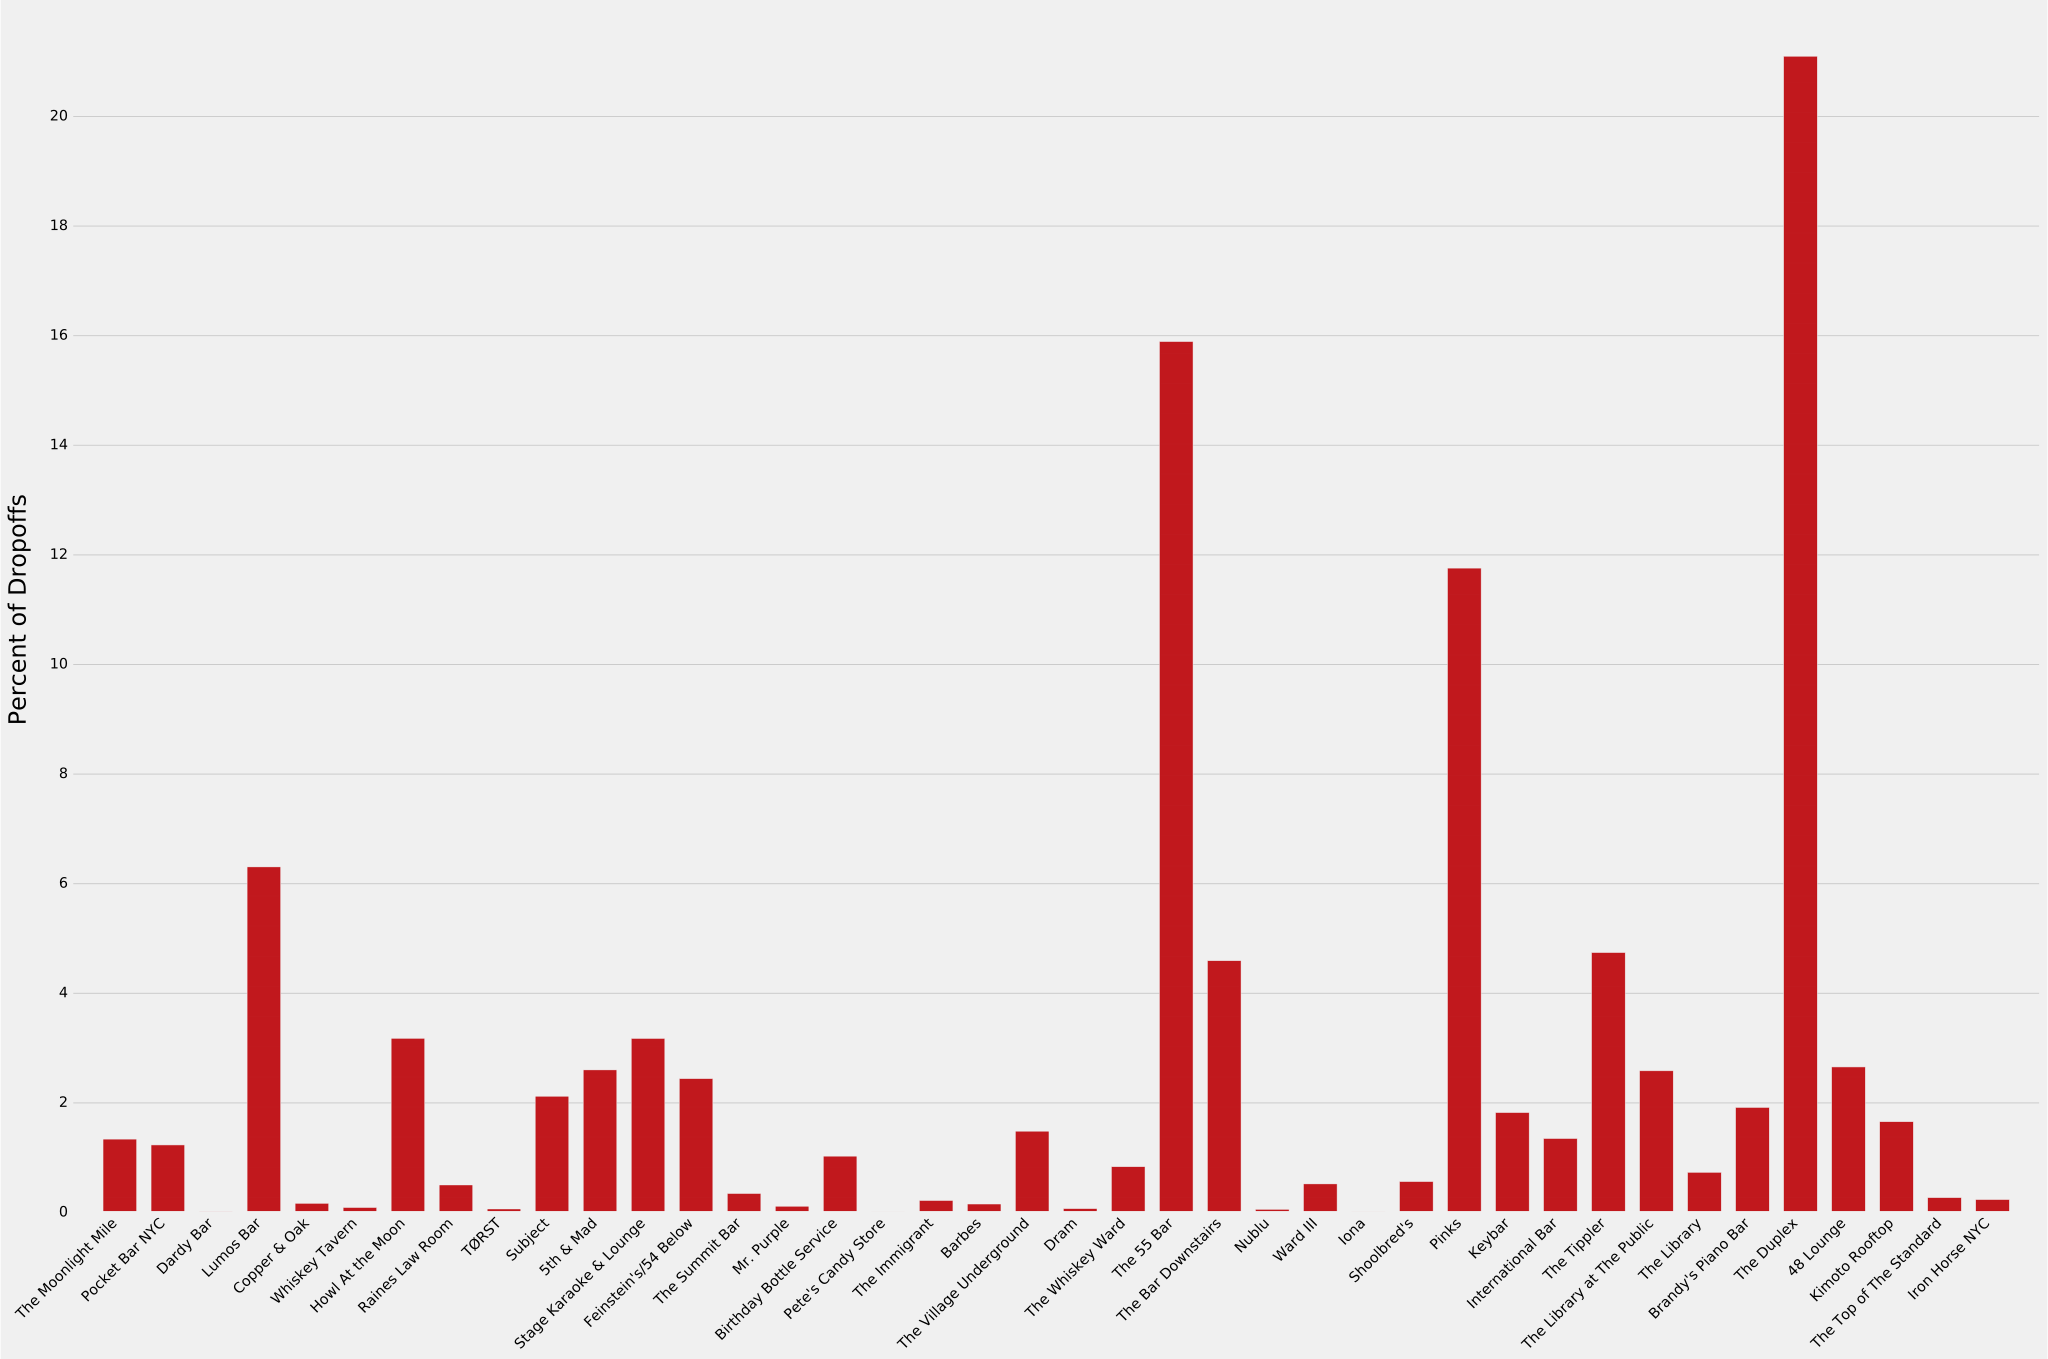
\includegraphics[scale=0.15]{nightlife}
\caption{Popularity of each venue based on number of dropoffs} 
\end{figure}
\end{frame}

\begin{frame}{New York Night Life}
\begin{figure}
\centering 
\includegraphics[scale=0.25]{NightlifeMapSize2}
\caption{Size of circle indicates percent of dropoffs} 
\end{figure}
\end{frame}

\section{Future Directions}
\begin{frame}{Future Directions}
\begin{itemize}
\item Examine correlations with other data sets
\begin{itemize}
\item Weather
\item Crime rates
\end{itemize}
\item A more sophisticated analysis of pickup and dropoff locations
\begin{itemize}
\item Cluster locations and see which restaurants, tourist attracts etc. fall into popular areas.
\item Filter based on time of day and day of week.
\item Correlation between number of dropoffs in area and future success of business 
\end{itemize}
\item Examine all six years worth of data to see trends over time
\end{itemize}
\end{frame}


\end{document}